\chapter{Sprint 2 - Design and implementation}

\section*{Introduction}
\addcontentsline{toc}{section}{Introduction}
In this chapter, we detail the objectives and functionalities of Sprint 2, which focuses on the Rental Order Management within the Odoo ERP system.

\section{Sprint 2 Backlog}
The Sprint 2 Backlog (Table \ref{tab:sprint2_backlog}) outlines tasks related to generating rental order reports with various view modes and filters, each task accompanied by its estimated duration, facilitating efficient sprint planning and resource allocation.

\begin{longtable}{|c|p{8cm}|c|}
    \hline
    \rowcolor{purple!20} \textbf{N°} & \textbf{Tasks} & \textbf{Duration} \\ \hline
    \endfirsthead
    \hline
    \rowcolor{purple!20} \textbf{N°} & \textbf{Tasks} & \textbf{Duration} \\ \hline
    \endhead
    1 & As an administrator, I can manage rental orders for products. & 3 Day \\ \hline
    2 & As a member, I can view my rental order history. & 1 Days \\ \hline
    3 & As an administrator, I can generate rental order reports. & 4 Day \\ \hline
    4 & As a member, I can reserve products for a specific date and time. & 6 Day \\ \hline
    5 & As an administrator, I can view and manage product reservations. & 3 Day \\ \hline
    6 & As an administrator, I can confirm or cancel reservations. & 1 Days \\ \hline
    7 & As an administrator, I can track stock levels for each product. & 6 Day \\ \hline
    8 & As an administrator, I can receive new stock shipments and update inventory. & 4 Day \\ \hline
    9 & As an administrator, I can set low stock alerts for products. & 2 Day \\ \hline
    10 & As an administrator, I can view the timeline of product rentals. & 3 Day \\ \hline
    11 & As an administrator, I can track rental durations and return dates. & 4 Day \\ \hline
    \caption{Sprint 2 Backlog for Rental Order Management, Stock Management, and Rental Timeline}
    \label{tab:sprint2_backlog}
\end{longtable}

\section{Functional Specifications}

\subsection{Use Case Diagram}
In this section, we present the functional specifications for the Rental Order Management module.
\newpage
\begin{figure}[h]
    \centering
    \makebox[\textwidth][c]{%
        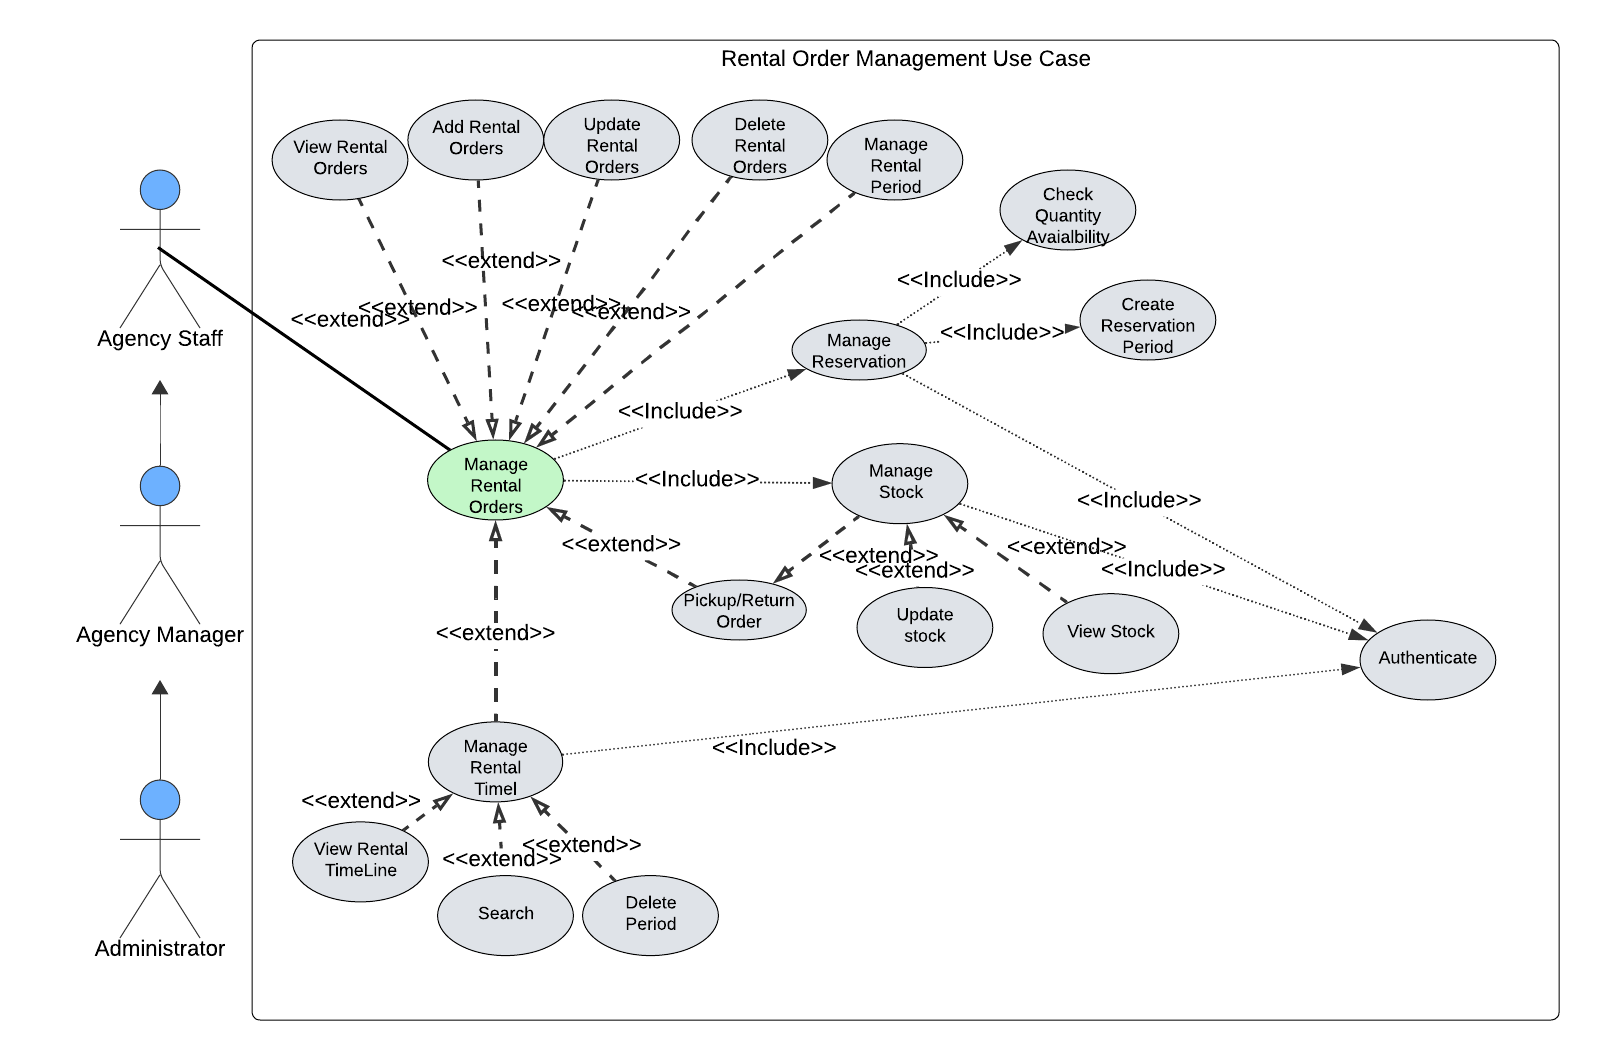
\includegraphics[width=1.2\textwidth]{sprint2/sprint2usecase.png}} % replace with your image path
    \caption{Use Case Diagram for Rental Order Management}
    \label{fig:sprint2_use_case_diagram}
\end{figure}

\subsection{Rental Order Sequence Diagram}
We present a dynamic model illustrating key scenarios of the most important use cases for Sprint 2 in the form of a sequence diagram. the process of creating a rental order:

\begin{itemize}
    \item The administrator initiates the creation of a new rental order.
    \item The system displays a rental order creation form.
    \item The administrator fills out the form with relevant details and submits it.
    \item The rental reservation model verifies and confirms the creation of the rental order.
    \item The system updates the rental stock based on the new order.
    \item The rental order state changes to reserved
    \item If the data is invalid or missing, the form remains in edit mode for correction.
    \item The administrator corrects and resubmits the data.
\end{itemize}

As depicted in Figure \ref{fig:rental_order_sequence_diagram}, the sequence diagram illustrates the "Rental Order Process" in detail.

\begin{figure}[h]
    \centering
    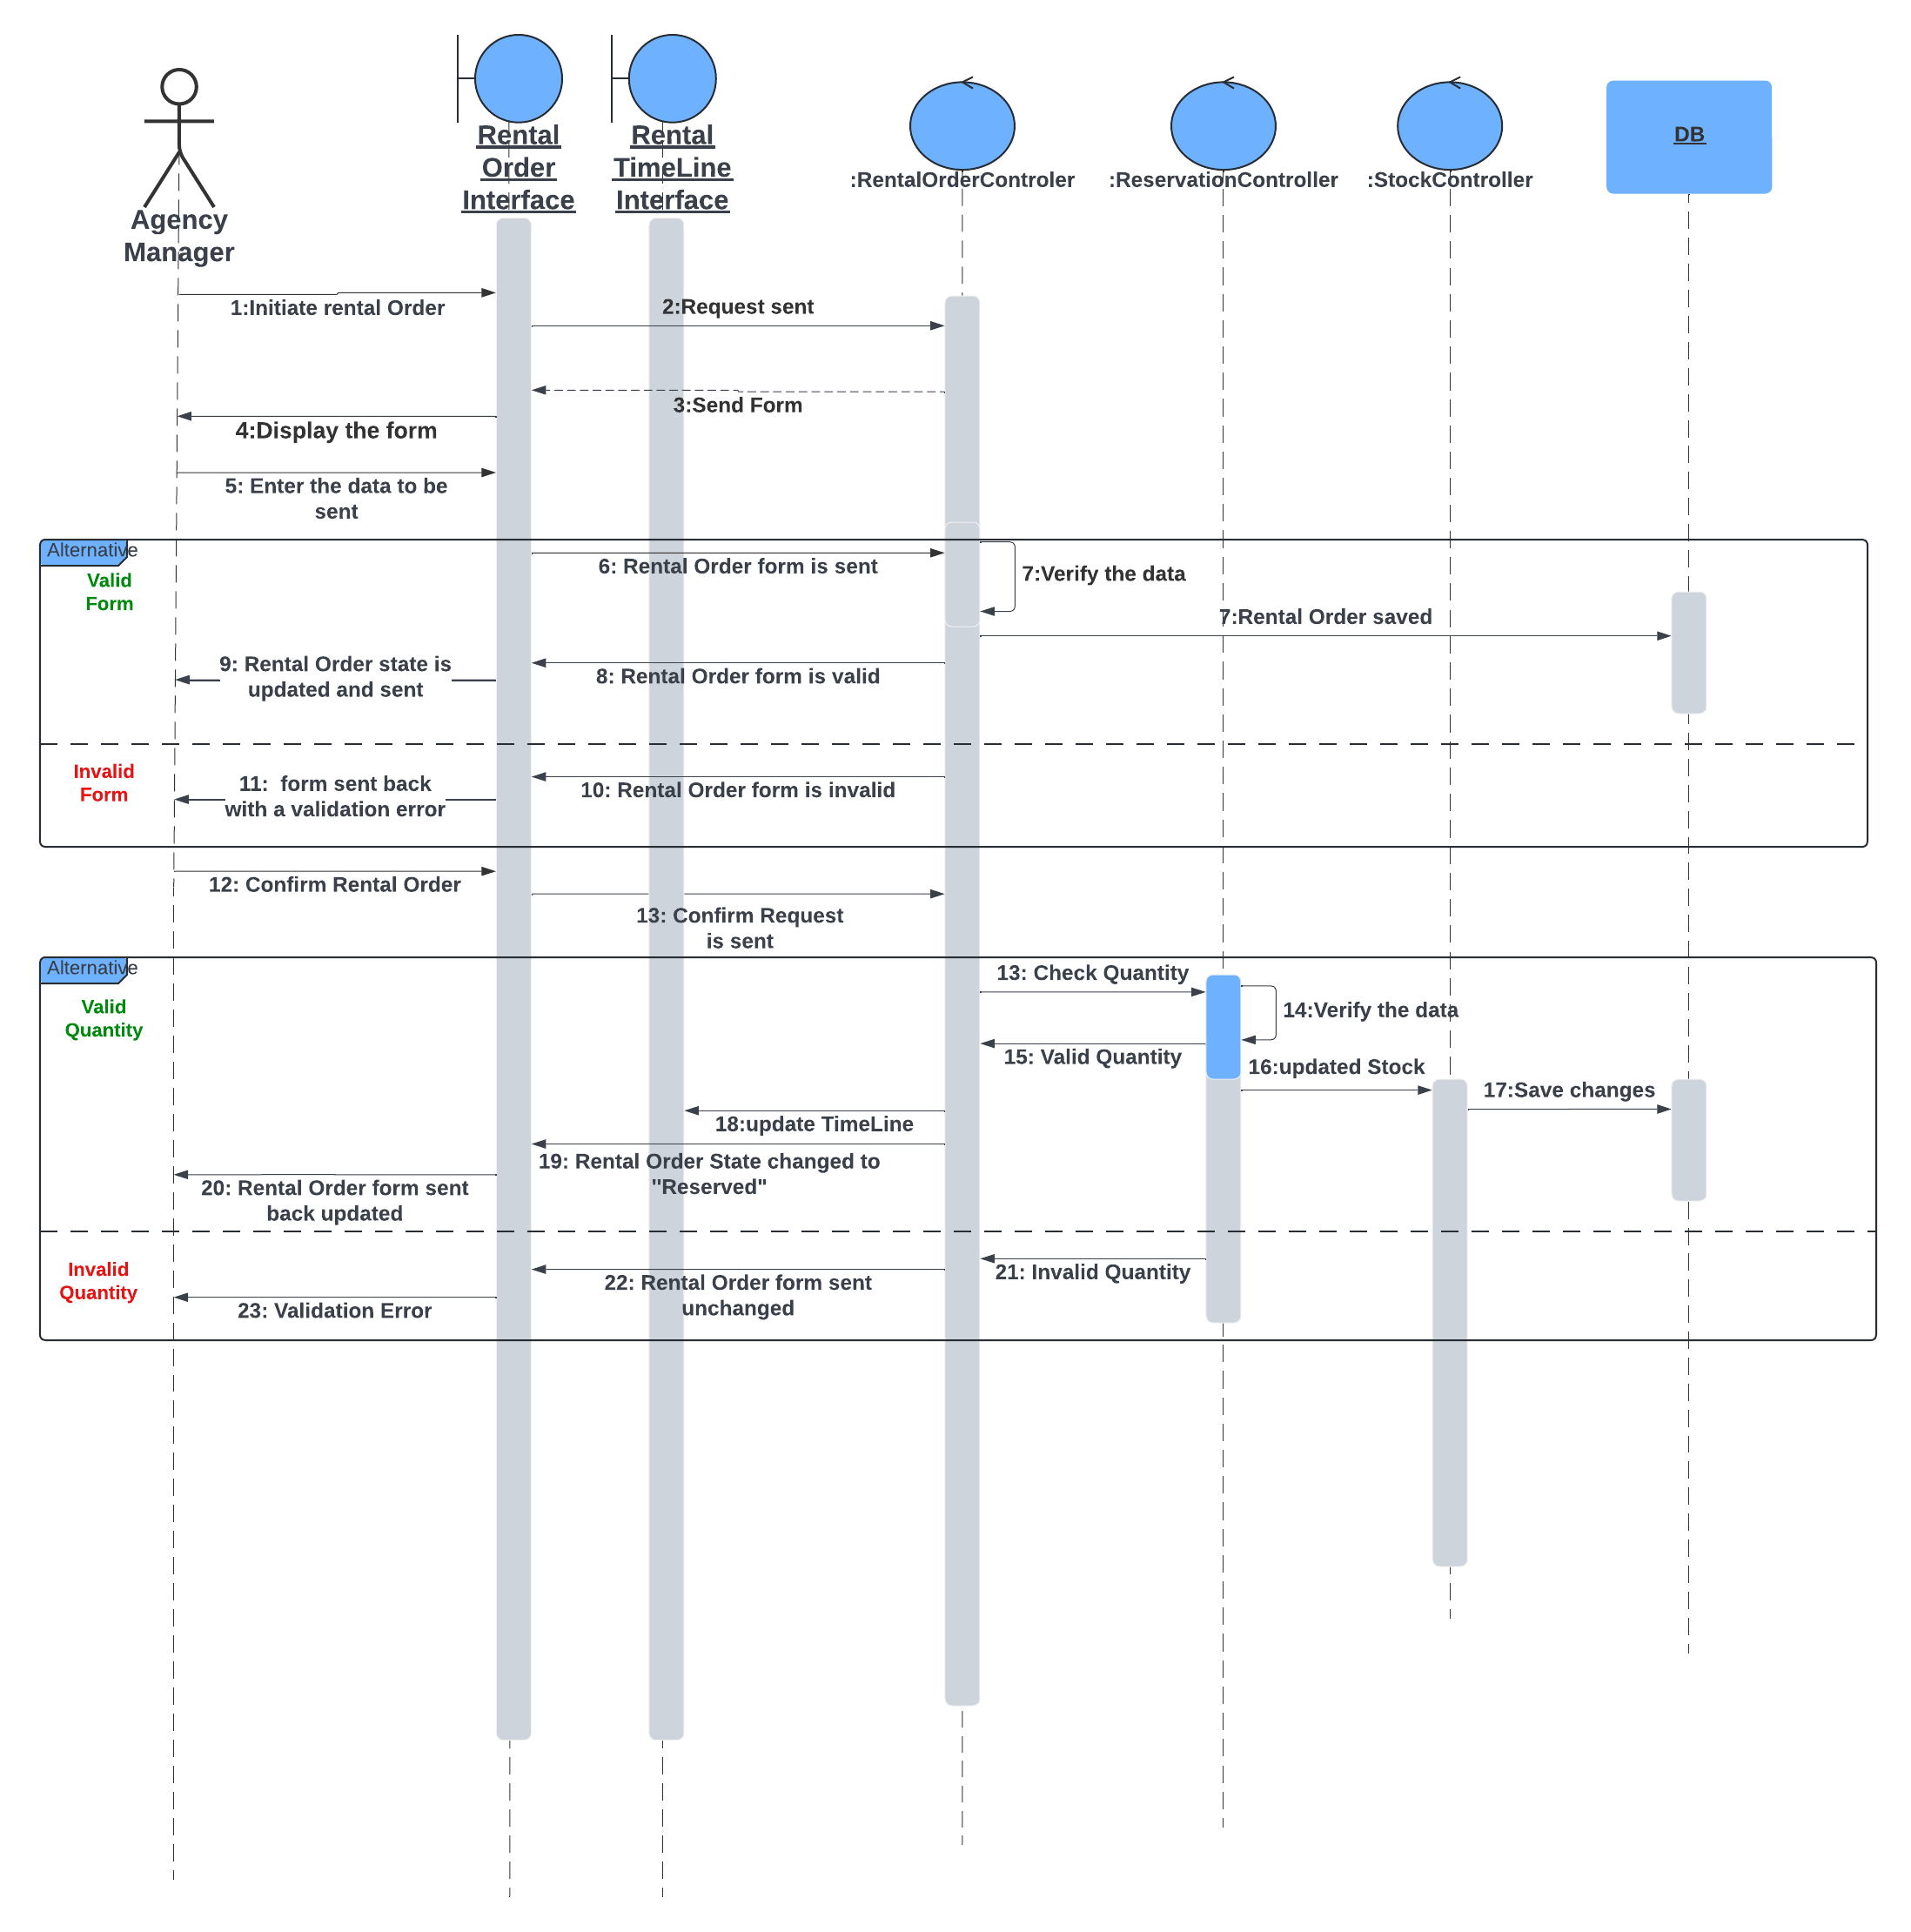
\includegraphics[width=1\textwidth]{sprint2/Sprint2Sequence1.png}
    \caption{Sequence Diagram for "Rental Order Process"}
    \label{fig:rental_order_sequence_diagram}
\end{figure} 
\newpage
\subsection{Pickup and Retur Order Sequence Diagram}

\begin{itemize}
    \item \textbf{Picking Up Rental Items:}
    \begin{itemize}
        \item The administrator initiates the pickup process for the rental order.
        \item The system displays the Pickup Order Wizard.
        \item The administrator specifies the quantities to be collected for each rental item.
        \item The system updates the rental stock to reflect the picked up quantities.
        \item The rental order state changes to rented if all items are picked up.
        \item If quantities are insufficient or other errors occur, the process handles alternatives.
    \end{itemize}
    \item \textbf{Returning Rental Items:}
    \begin{itemize}
        \item The administrator initiates the return process for the rental order.
        \item The system displays the Return Order Wizard.
        \item The administrator specifies quantities to be returned for each rental item.
        \item The system updates the rental stock to reflect the returned quantities and return dates.
        \item The rental order state changes to done if all items are returned.
        \item If quantities are insufficient or other errors occur, the process handles alternatives.
    \end{itemize}
\end{itemize}
\newpage
As shown in Figure \ref{fig:pickup_return_ordersequence_diagram}, the sequence diagram depicts the process of "Pickup/Return" orders.

\begin{figure}[h]
    \centering
    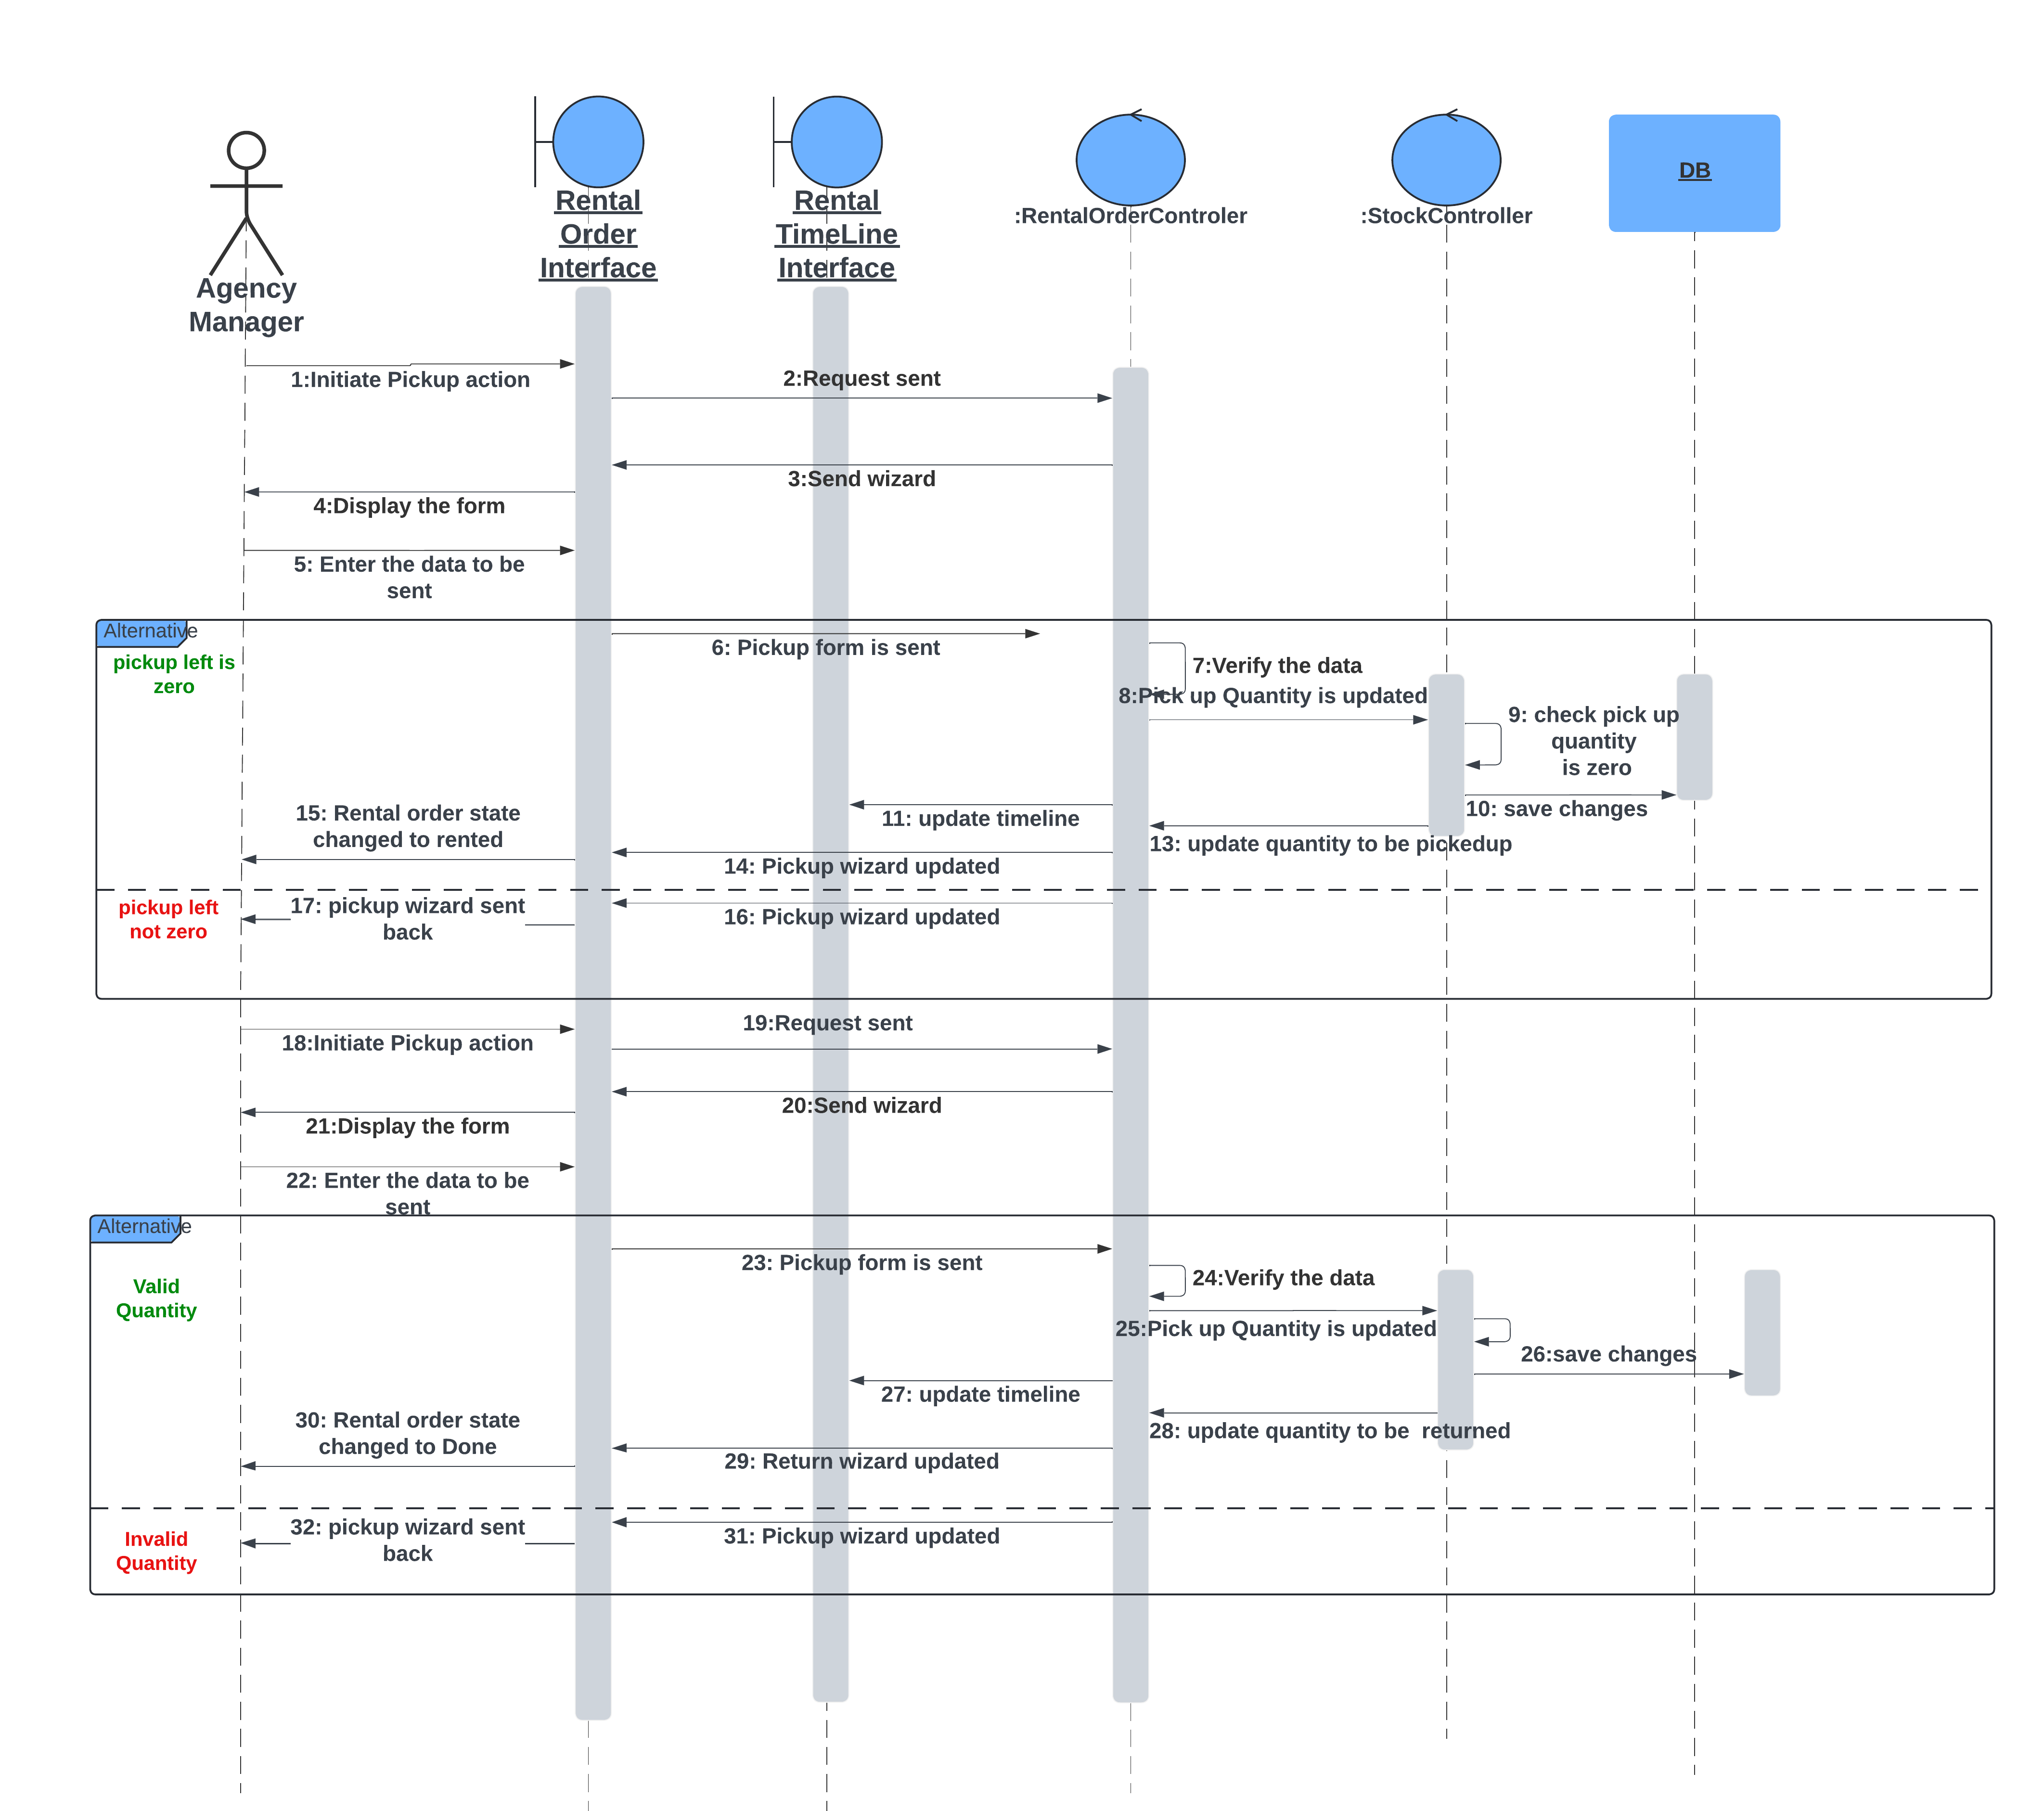
\includegraphics[width=1\textwidth]{sprint2/Sprint2Sequence2.png}
    \caption{Sequence Diagram for "Pickup/Return" Order}
    \label{fig:pickup_return_ordersequence_diagram}
\end{figure}

\section{Sprint Realization}
\subsection{Rental Order Form}
The screenshot in Figure \ref{fig:rental_order_form} displays the initial rental order form where the administrator fills out details such as customer information, rental duration, and selected products.
\newpage
% \begin{figure}[h]
%     \centering
%     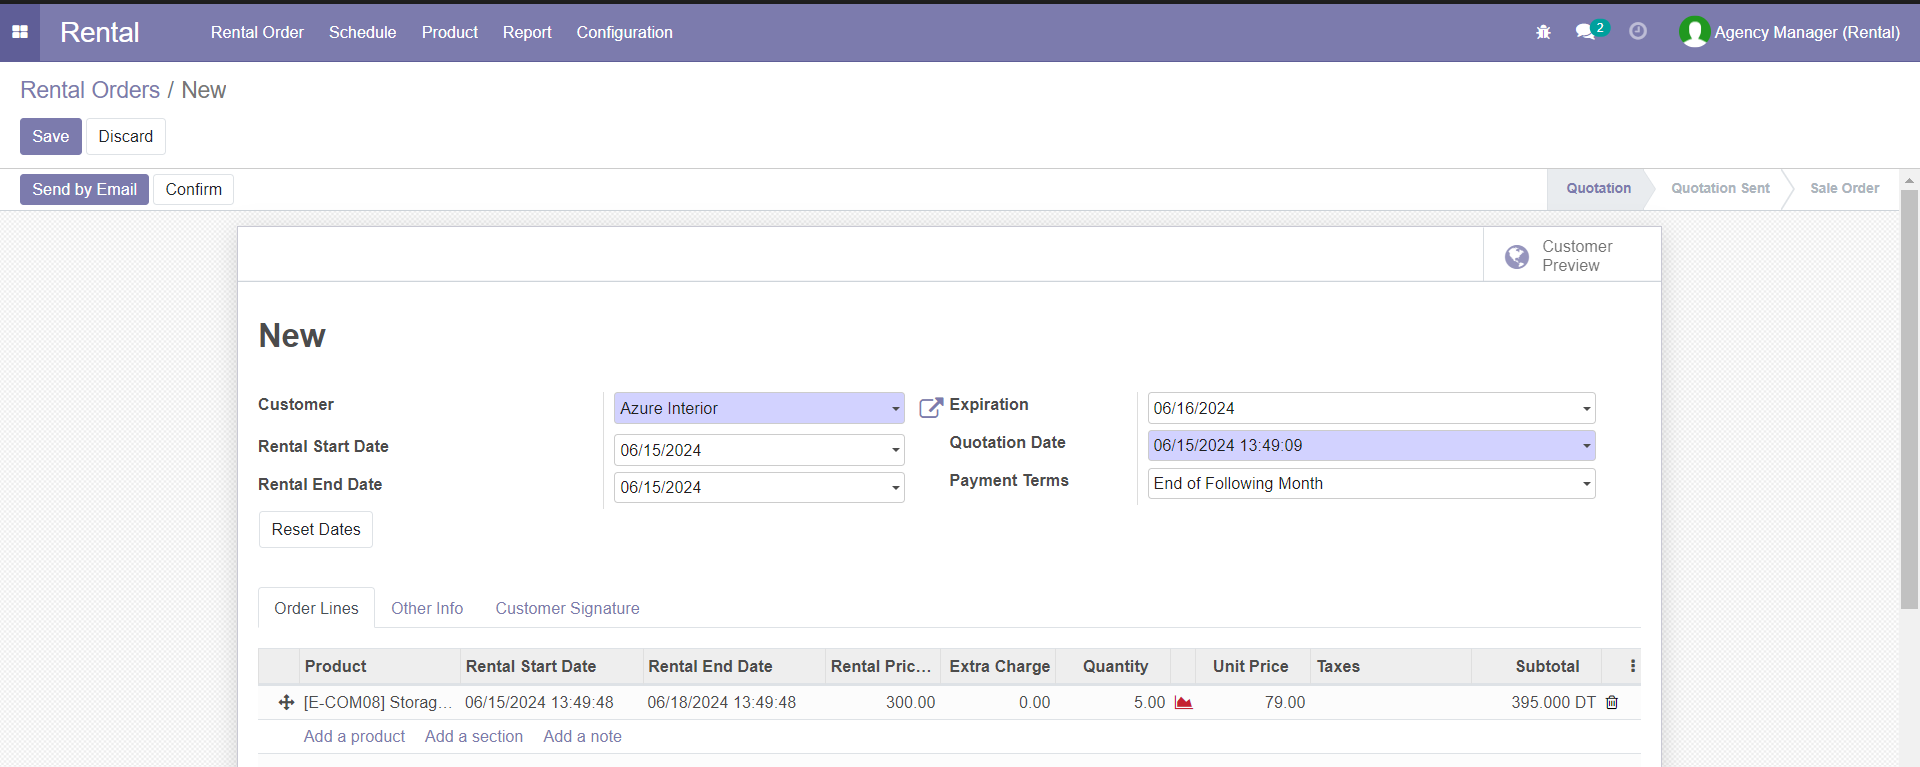
\includegraphics[width=1\textwidth]{sprint2/rentalorder1.png}
%     \caption{Screenshot of Rental Order Form}
%     \label{fig:rental_order_form}
% \end{figure}
\begin{figure}[h]
    \centering
    \makebox[\textwidth][c]{%
        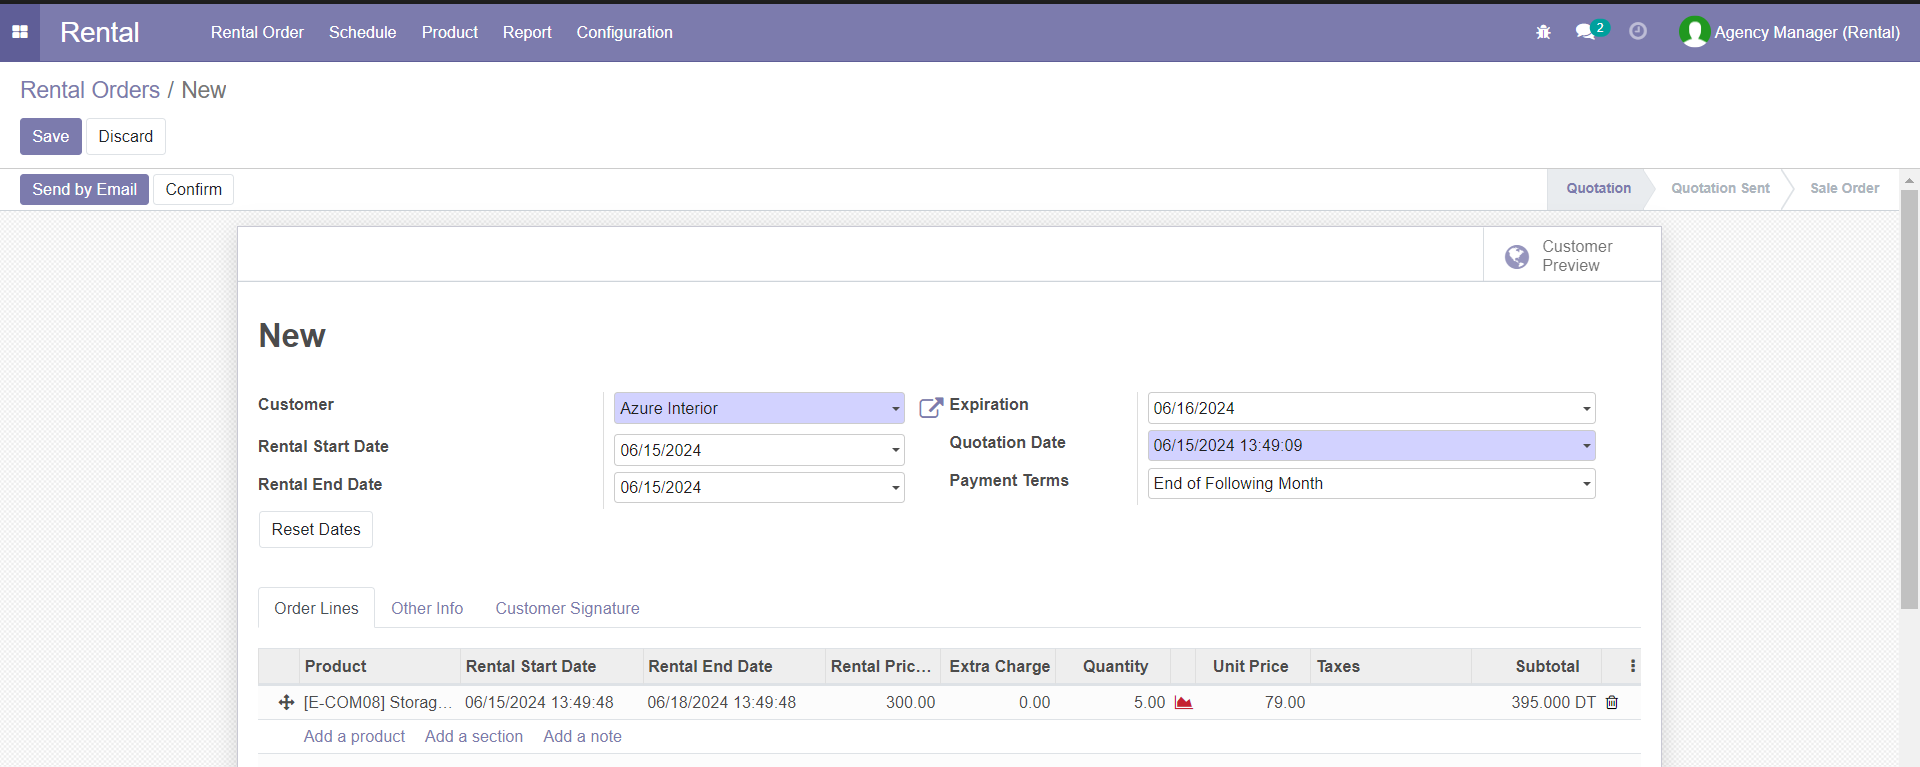
\includegraphics[width=1.2\textwidth]{sprint2/rentalorder1.png}} % replace with your image path
    \caption{Screenshot of Rental Order Form}
    \label{fig:rental_order_form}
\end{figure}

\subsection{Confirmed Rental Order}
Figure \ref{fig:confirmed_rental_order} illustrates the confirmation screen of the rental order after submission. It indicates successful validation and reservation of rental items.

% \begin{figure}[h]
%     \centering
%     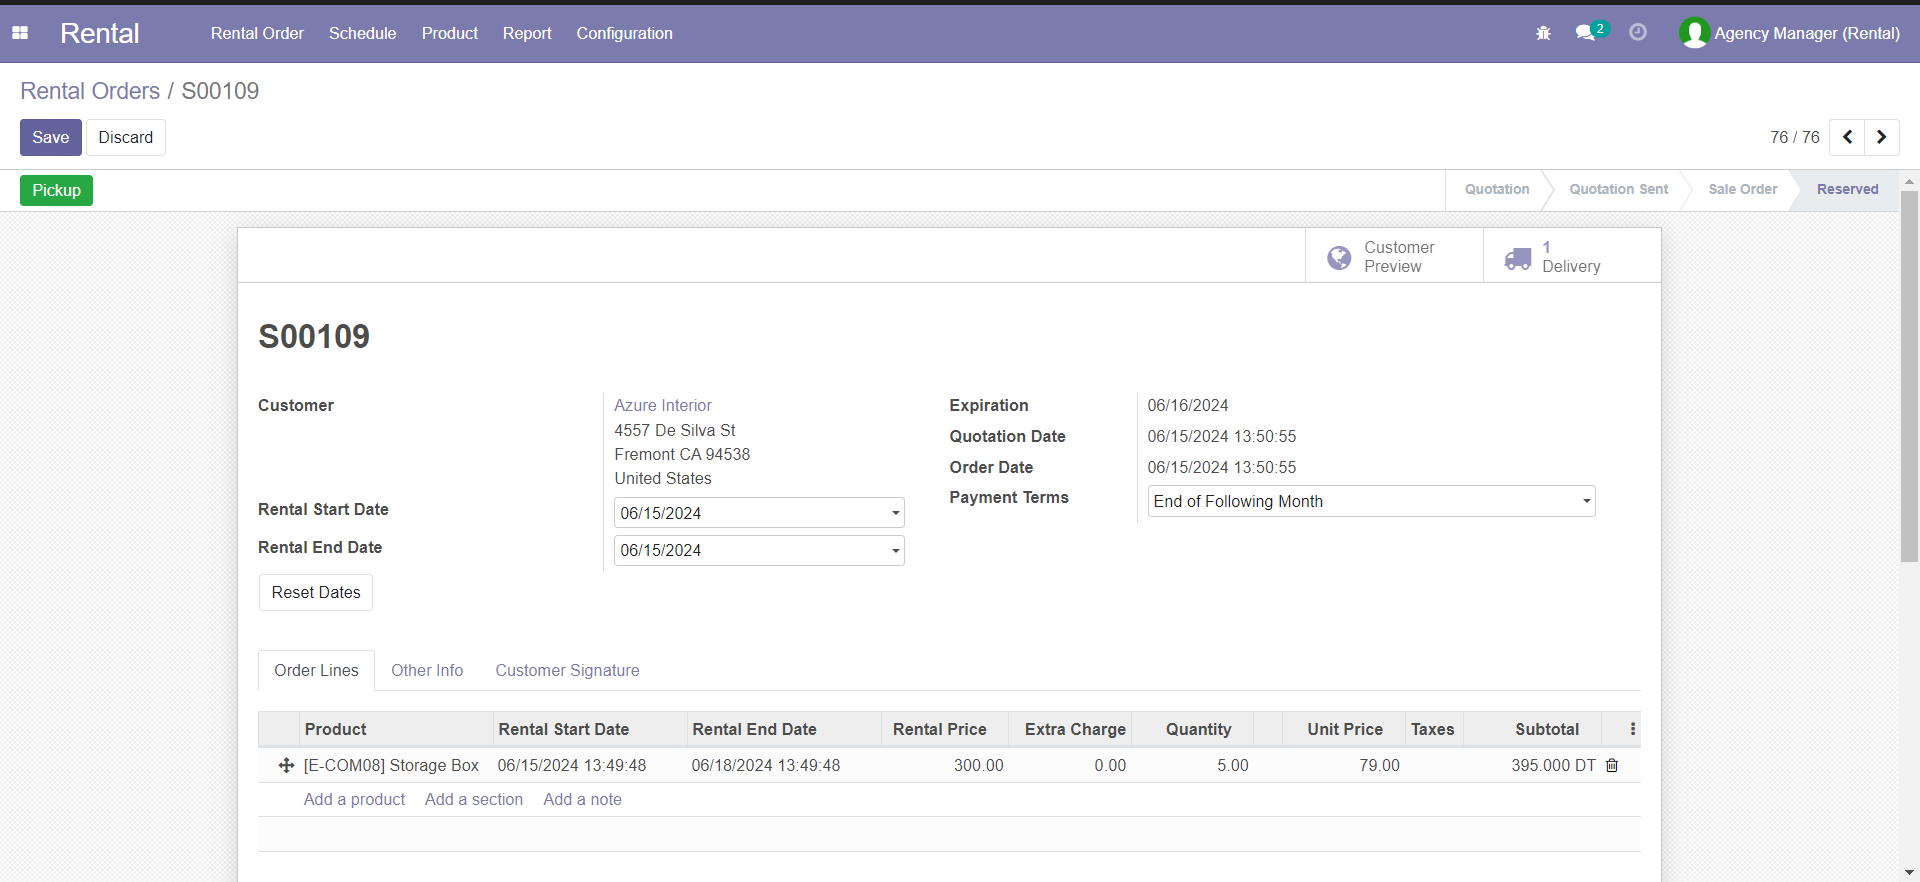
\includegraphics[width=1\textwidth]{sprint2/rentalorder2.png}
%     \caption{Screenshot of Confirmed Rental Order}
%     \label{fig:confirmed_rental_order}
% \end{figure}
\begin{figure}[h]
    \centering
    \makebox[\textwidth][c]{%
        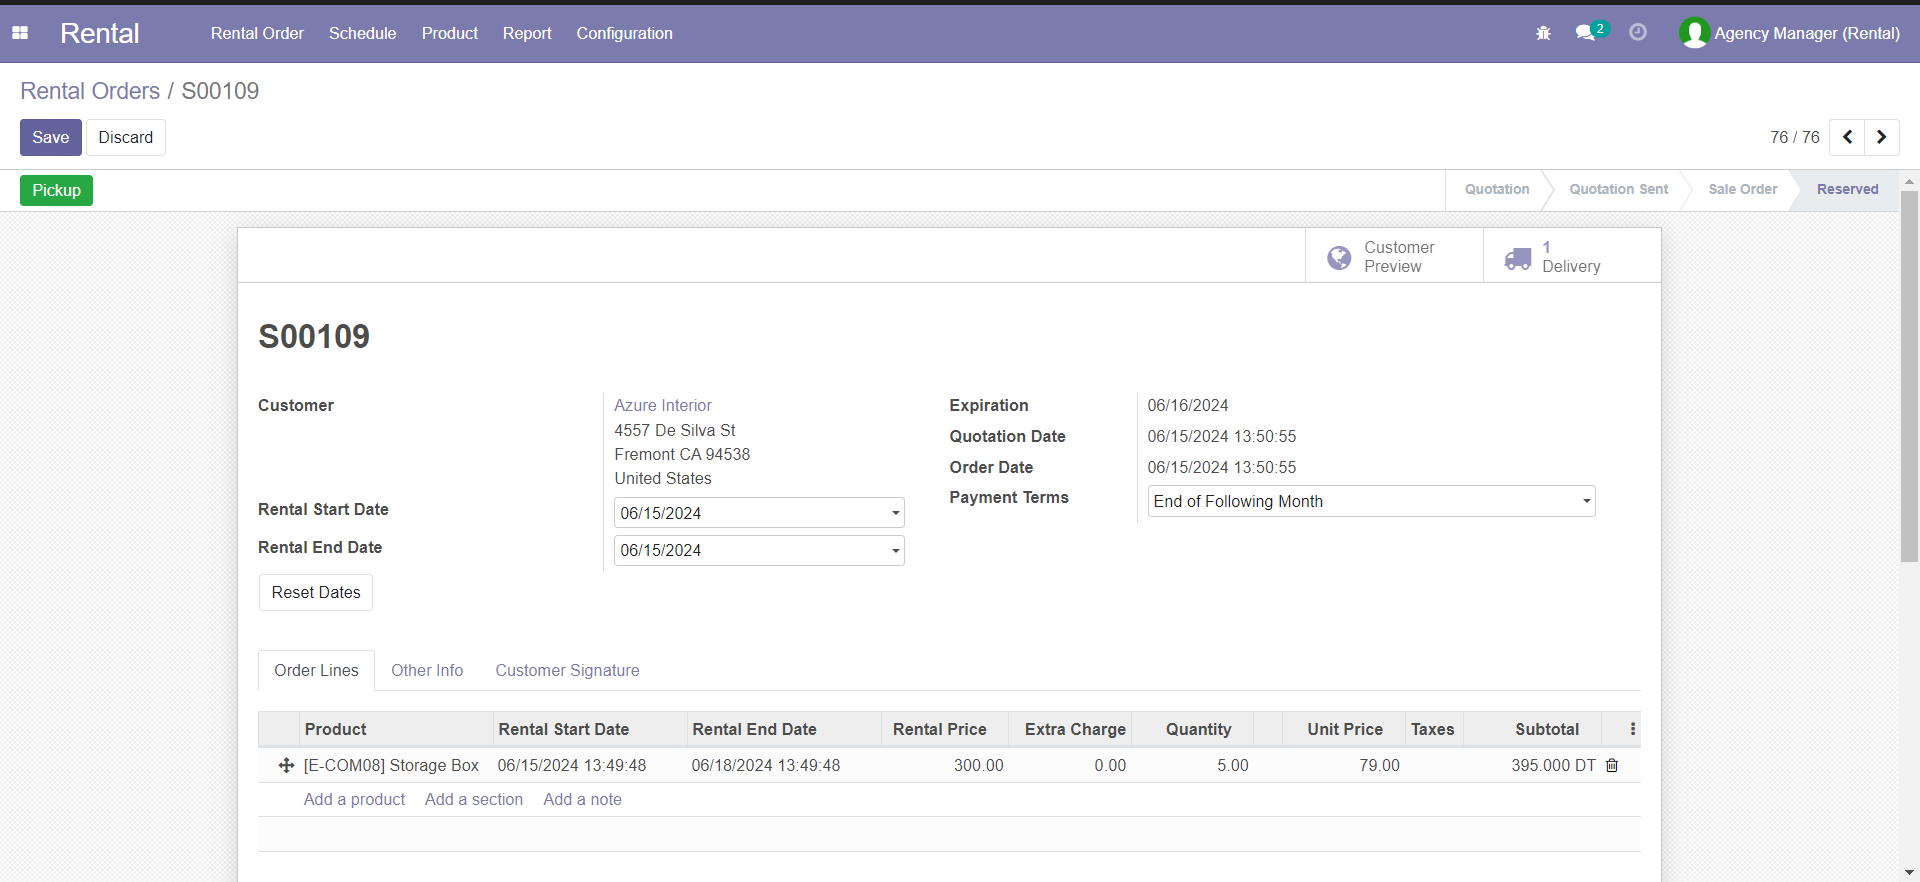
\includegraphics[width=1.2\textwidth]{sprint2/rentalorder2.png}} % replace with your image path
    \caption{Screenshot of Confirmed Rental Order}
    \label{fig:confirmed_rental_order}
\end{figure}

\subsection{Pickup Wizard}
Figure \ref{fig:pickup_state} shows the Pickup Wizard where the administrator manages quantities for pickup, updating the rental stock and changing the rental order state to rented (green).

\begin{figure}[h]
    \centering
    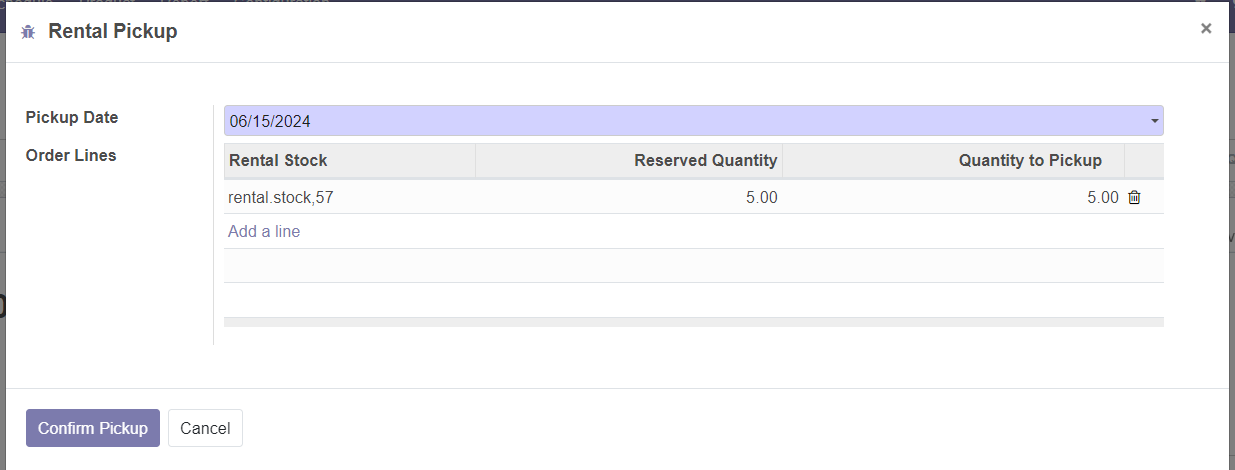
\includegraphics[width=1\textwidth]{sprint2/rentalorderpickup3.png}
    \caption{Screenshot of Pickup State}
    \label{fig:pickup_state}
\end{figure}

\subsection{Return Wizard}
Figure \ref{fig:return_state} shows the Return Wizard where the administrator manages returns, calculates any extra charges for late returns, updates the stock, and changes the rental order state to done (grey).

\begin{figure}[h]
    \centering
    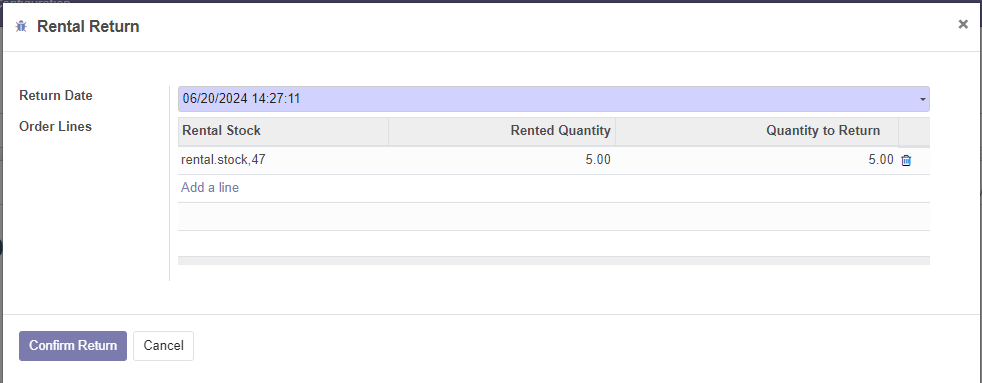
\includegraphics[width=1\textwidth]{sprint2/rentalorderreturn4.png}
    \caption{Screenshot of Return State}
    \label{fig:return_state}
\end{figure}

\subsection{Rental Stock Movement}
Figure \ref{fig:rental_stock_view} visualizes the movements of rental stock items, Each item is associated with its order ID for tracking. The stock view shows quantity updates as rental orders change.
\begin{figure}[h]
    \centering
    \makebox[\textwidth][c]{%
        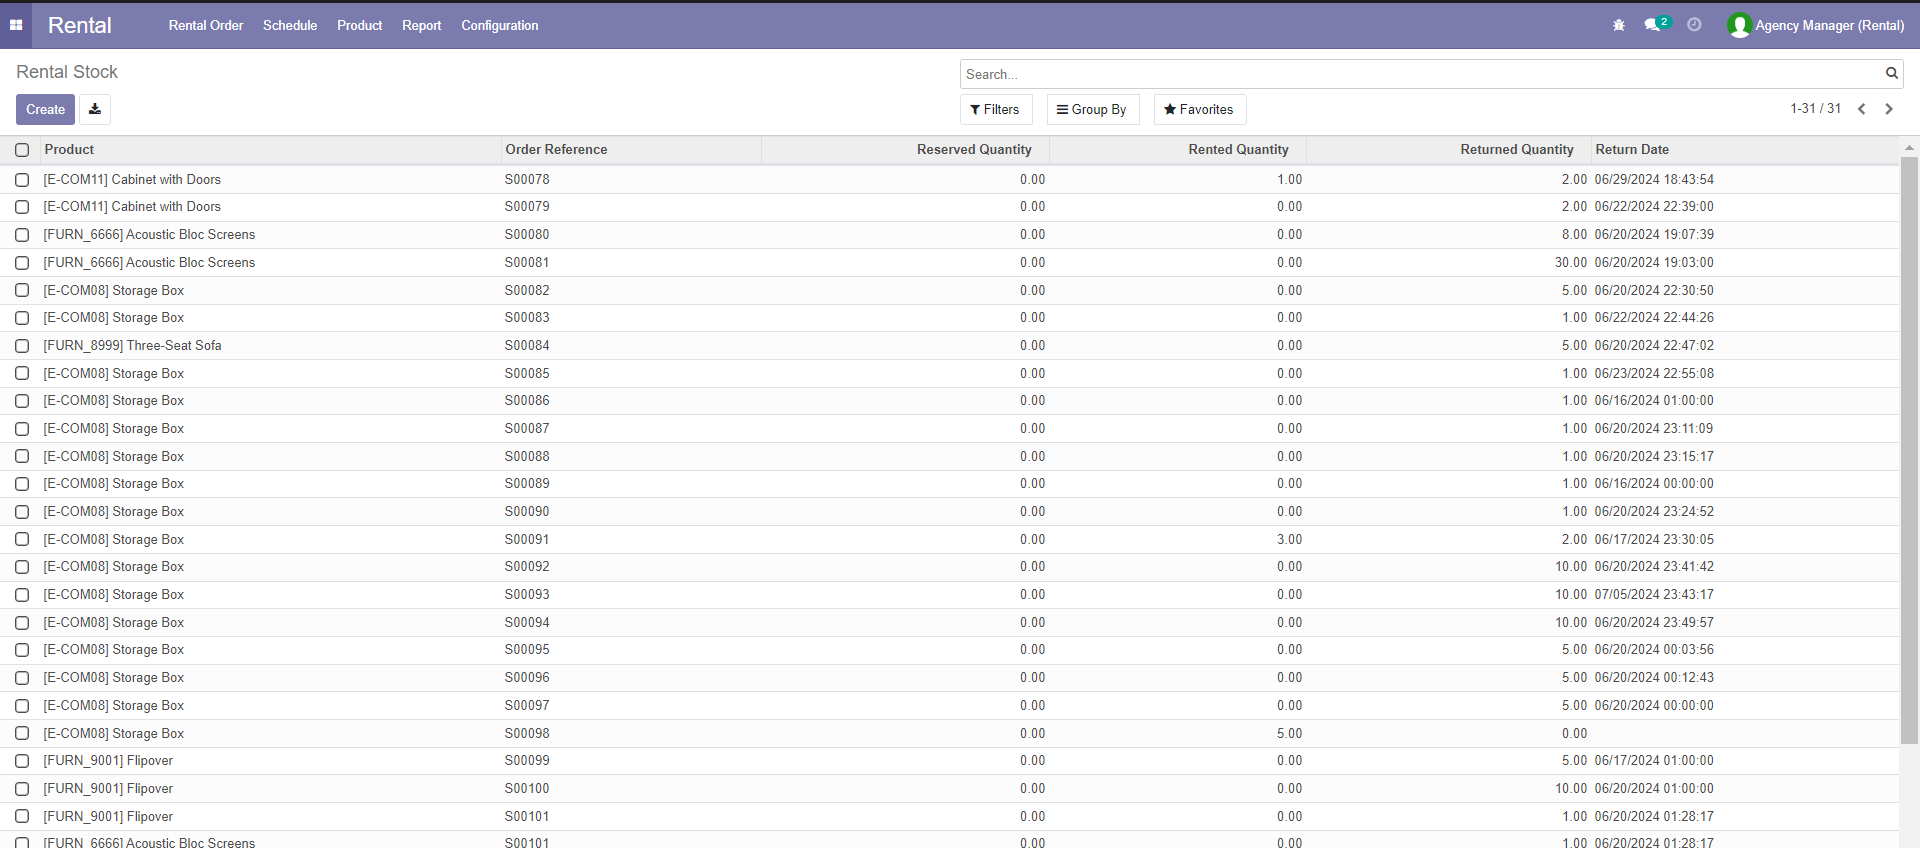
\includegraphics[width=1.2\textwidth]{sprint2/rentalorderstock7.png}} % replace with your image path
    \caption{Rental Stock View}
    \label{fig:rental_stock_view}
\end{figure}

\subsection{Rental Schedule Timeline}
Figure \ref{fig:rental_schedule_timeline} illustrates the rental schedule timeline, showing how information is grouped by product. It highlights the progress of each order through different states—reserved (blue), rented (green), and done (grey)—and includes the associated order ID for reference. The timeline updates reflect changes in rental orders.

% \begin{figure}[h]
%     \centering
%     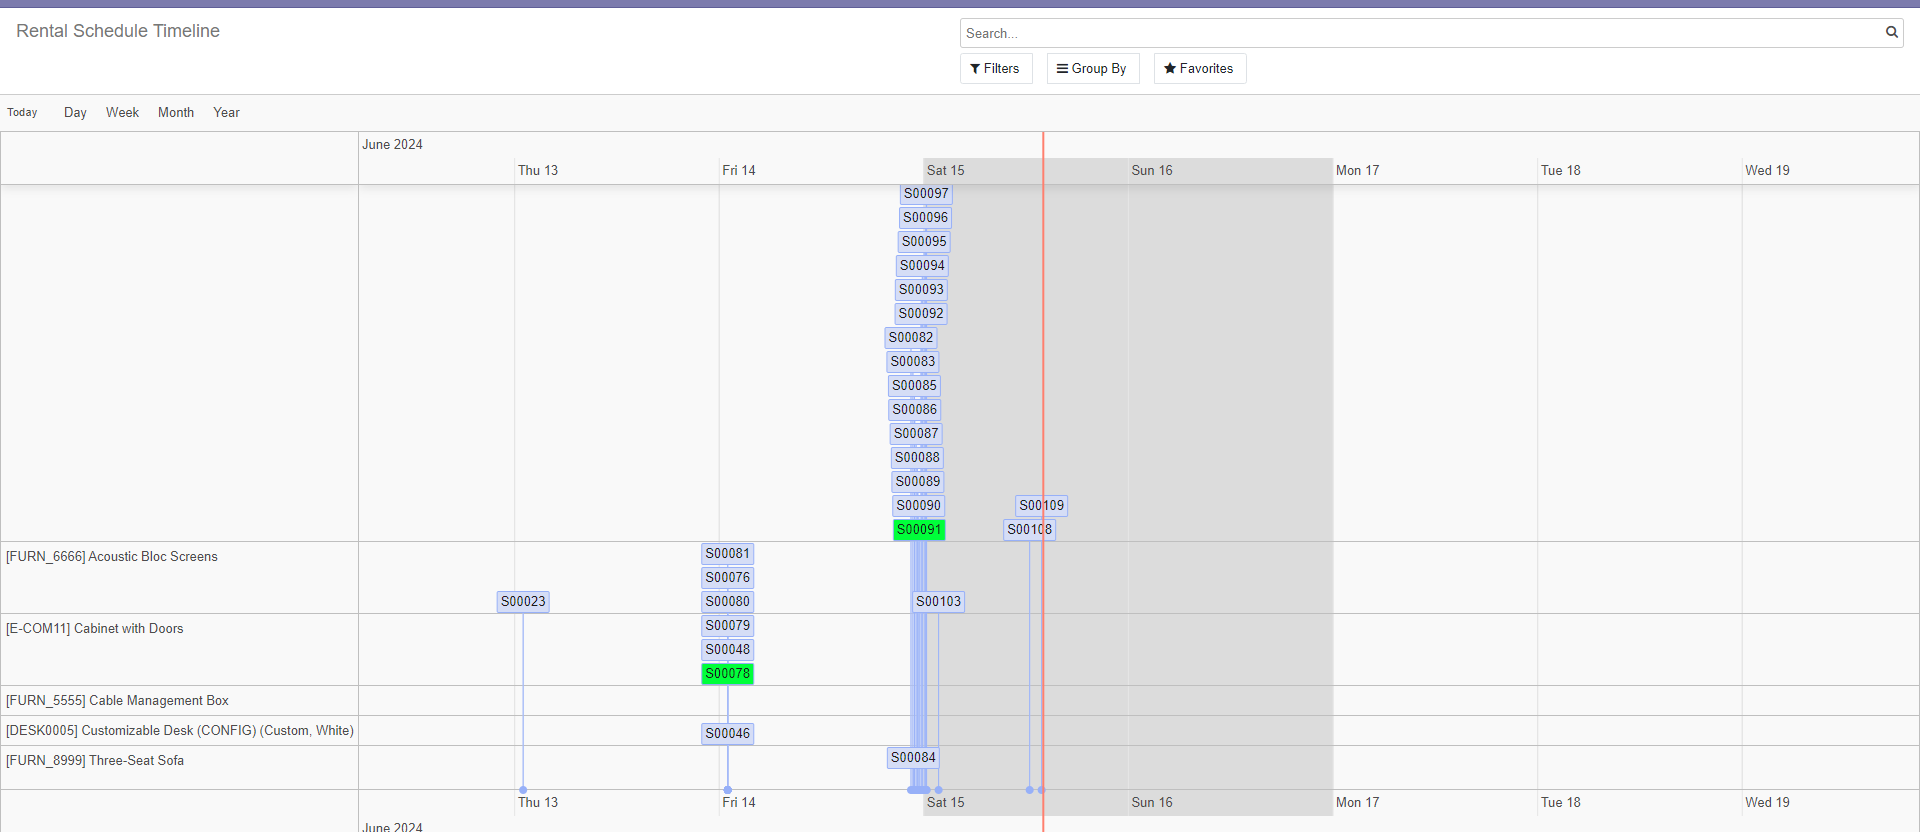
\includegraphics[width=1\textwidth]{sprint2/rentalorderschedule6.png}
%     \caption{Screenshot of Timeline}
%     \label{fig:rental_schedule_timeline}
% \end{figure}
\begin{figure}[h]
    \centering
    \makebox[\textwidth][c]{%
        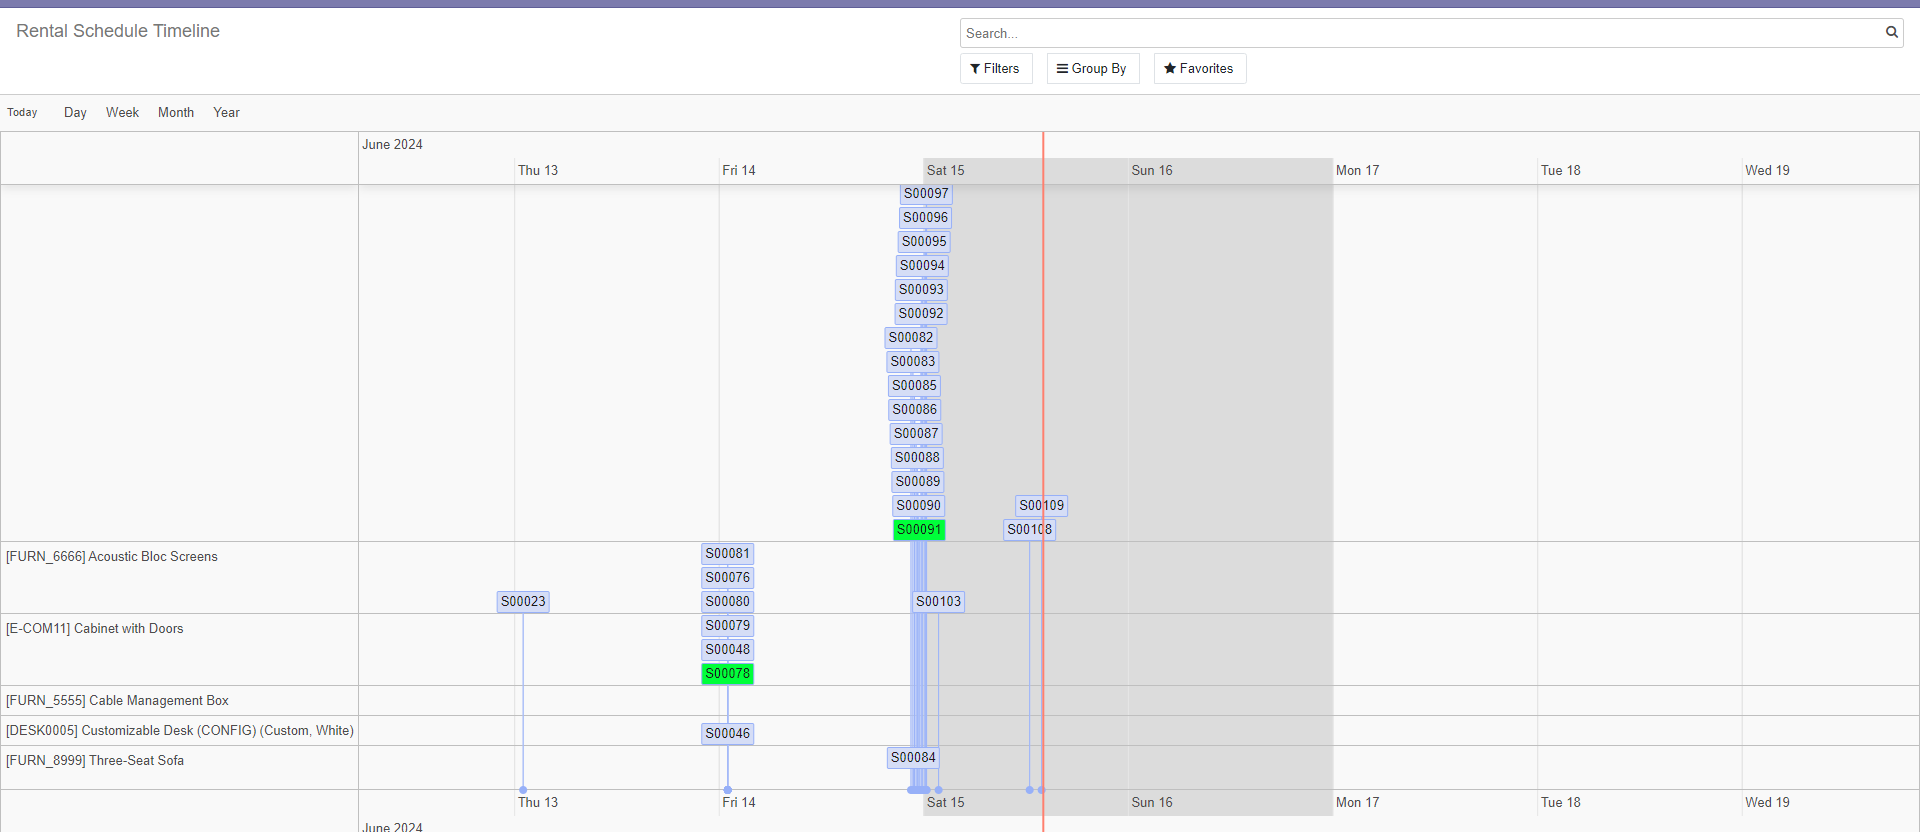
\includegraphics[width=1.1\textwidth]{sprint2/rentalorderschedule6.png}} % replace with your image path
    \caption{Screenshot of Timeline}
    \label{fig:rental_schedule_timeline}
\end{figure}
\newpage
\section*{Conclusion}
\addcontentsline{toc}{section}{Conclusion}

In Sprint 2, we established key functionalities in the rental order process module of Odoo ERP. This included the "Order Details," "Inventory Management," and "Rental Pricing" notebooks, along with the "Update Order Status" button and "Order Status" display, enhancing the rental order management process. In the next sprint, we will focus on integrating the rental order process with billing and invoicing to streamline financial operations.
